\chapter{AGN \& Quasars}

\section{Active Galactic Nuclei}

Active Galactic Nuclei (AGN  \footnote{Notes for this section taken from \href{https://www.isdc.unige.ch/~ricci/Website/Active_Galactic_Nuclei.html}{\textcolor{blue}{here}}} ) are the most luminous persistent sources of radiation in the Universe, and are powered by accretion onto a supermassive black hole (SMBH). In the last ten years it has become evident that most galaxies have gone through an AGN phase, which has played a crucial role in their formation and evolution. The typical AGN is made of several components (see Fig. \ref{fig:agn_schematic}):

\begin{enumerate}
    \item An accretion disk where matter is funneled onto the SMBH.
    \item A broad line region (BLR) where the broad and optical/UV lines are produced. Reverberation mapping studies have shown that the inner radius of this region scales with the luminosity and is  ~10-100 light days (e.g., Kaspi et al. 2005).
    \item A molecular torus, which is located within few parsecs from the SMBH. Near-IR reverberation studies have shown that the inner radius of the torus also scales with the luminosity (Suganuma et al. 2006).
    \item A narrow line region (NLR), which is located at ~100-300 pc from the SMBH, where the narrow optical lines are created.

\end{enumerate}

\section{Types of AGN }
Most AGN are radio-quiet, and can be divided into two classes \footnote{Kind of a misnomer- it doesn't mean there are two types of AGN, just means we have different viewing angles.}, according to their optical spectra. Type-I AGN, also called Seyfert 1s (Sy1s), show both broad and narrow lines, while type-II AGN (Seyfert 2s or Sy2s) show only narrow lines (see Fig. \ref{fig:seyfert_spectra}, taken from \href{https://reader.elsevier.com/reader/sd/pii/S1387647300000658?token=660DD777DEA7E41F7AD39364C79E4FA98C1E0C5C81431C48635052498601540CC37DC9AC7BA43B3AADF61AA5A59524EB&originRegion=eu-west-1&originCreation=20230127115455}{Pogge, 2000}). \\
\\
According to the simple unification model (e.g., Antonucci 1993), these objects are intrinsically the same, but are observed with different inclination angles with respect to the molecular torus (Fig. 3). \\
\colorbox{yellow}{Type-I are observed pole on, so that it is possible to observe both the BLR and the NLR, while} \\
\colorbox{yellow}{type-II are see edge-on, and the BLR is hidden by the torus.}

It is easier to discover a large number of Seyfert I in X-rays because 


Optical and soft X-ray surveys alone are highly biased toward only unobscured AGNs, while this simple WISE selection likely identifies even heavily obscured, Compton-thick AGNs.



\begin{figure}
    \centering
    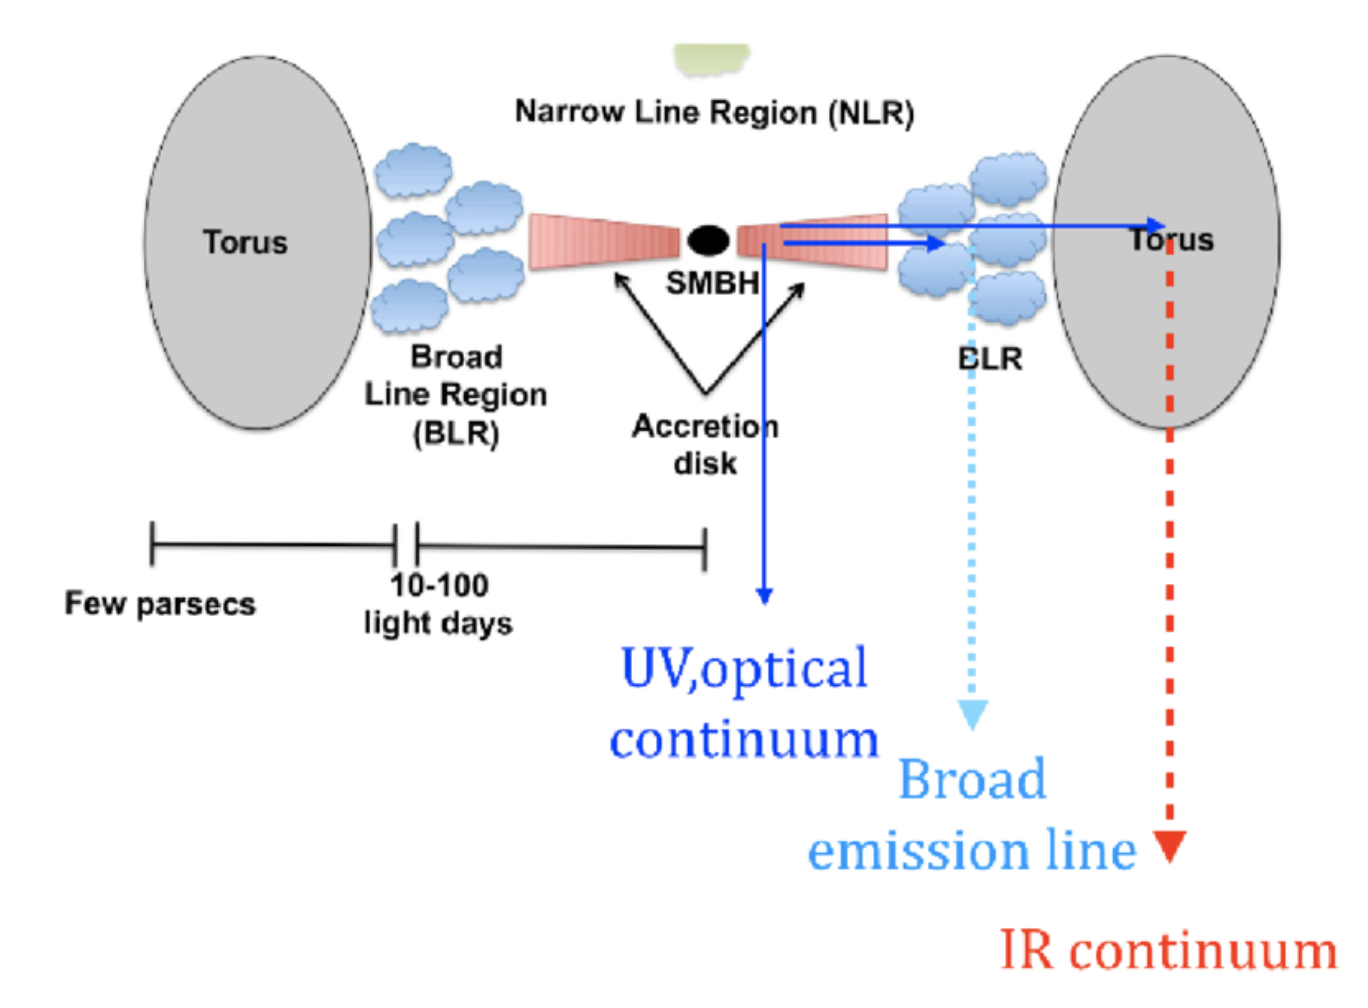
\includegraphics[scale=0.6]{Notes_Images/AGN_Schematic.png}
    \caption{Schematic diagram of the central structure of an AGN. Using the time lags among the light in different wavelengths, we will be able to estimate the physical size of each component (Image credit : Claudio Ricci)  }
    \label{fig:agn_schematic}
\end{figure}

\begin{figure}
    \centering
    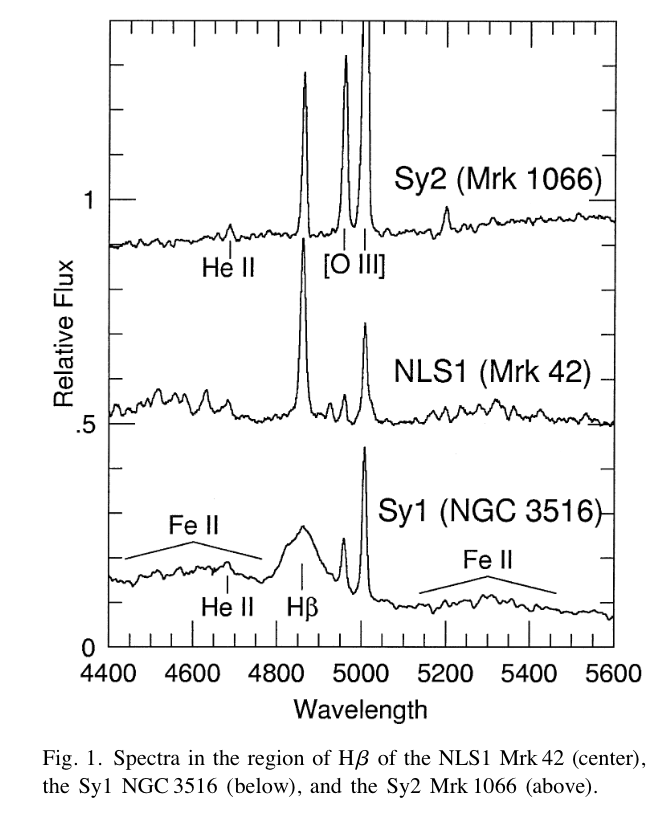
\includegraphics{Notes_Images/SeyfertsSpectra_Pogge.png}
    \caption{Spectra in the region of Hb of the NLS1 Mrk 42 (center),
the Sy1 NGC 3516 (below), and the Sy2 Mrk 1066 (above) taken from \href{https://reader.elsevier.com/reader/sd/pii/S1387647300000658?token=660DD777DEA7E41F7AD39364C79E4FA98C1E0C5C81431C48635052498601540CC37DC9AC7BA43B3AADF61AA5A59524EB&originRegion=eu-west-1&originCreation=20230127115455}{Pogge 2000}}
    \label{fig:seyfert_spectra}
\end{figure}

\section{Quasars}

\colorbox{yellow}{All quasars are AGNs, but not all AGNs are quasars.}\\
\\
 \href{https://arxiv.org/pdf/2007.12026.pdf}{Yesuf \& Ho 2020} : A recent far-infrared study indicates that \textbf{the gas content of the host galaxies of type 1 and type 2 quasars are similar}, and neither type is gas-deficient relative to normal, inactive galaxies (Shangguan \& Ho 2019). This is supported by the work of Zhuang \& Ho (2020), which is also based on the method of Yesuf \& Ho (2019).

\section{Hosts of AGN}
Griffith \& Stern 2010 find that the radio-selected AGNs are likely to be hosted by early-type galaxies, while X-ray- and mid-infrared-selected AGNs are more often associated with \textbf{point sources} and \textbf{disk galaxies}. 